\chapter{Ladesysteme}
Ein \emph{Ladesystem} ist ein technisches System, das elektrische Energie aus dem öffentlichen Stromnetz in den Energiespeicher des Busses transportiert. Die \emph{Ladestrategie} beschreibt, wann, wo und wie lange geladen wird. Es kann über Nacht im Depot ("`Nachtladung"'), oder tagsüber an Haltestellen beziehungsweise während der Fahrt geladen werden ("`Gelegenheitsladen"').\marginpar{Eventuell nochmal aufteilen in Ende der Tour – während der Fahrt?}

Im  Abschnitt \ref{untersuchte_Systeme} werden Funktionsweise und Einsatzgeschichte der verschiedenen Ladesysteme erläutert. Im Abschnitt \ref{parameter} werden die betrachteten technischen Parameter, die in dieser Arbeit zum Vergleich der Systeme herangezogen werden, vorgestellt und definiert. In Abschnitt \ref{sec_tabellen_ladesysteme} ab werden dann die für die verschiedenen Ladesysteme ermittelten Parameter tabellarisch aufgelistet. 

Viele technisch mögliche Kombinationen von Ladesystem und Ladestrategie machen betrieblich keinen Sinn – zum Beispiel der Einsatz eines aufwändigen Schnellladesystems für die Nachtladung im Depot. In dieser Arbeit werden Ladesysteme zusammen mit der für dieses System sinnvollen Ladestrategie betrachtet.

\section{Kategorisierung der Systeme}
Die Ladesysteme werden lassen sich nach den folgenden drei Kriterien kategorisieren:

\paragraph{Energietransport}
\begin{itemize}
	\item Konduktiv – elektrisch leitende Verbindung zwischen Bus und Ladestation
	\item Induktiv – Ladestation erzeugt Magnetfeld, das im Bus in Strom umgewandelt wird
	\item Batteriewechsel – die Batterie wird ausgewechselt
\end{itemize}

\paragraph{Fahrzustand}
\begin{itemize}
	\item Statisch – es wird nur geladen, während der Bus steht
	\item Dynamisch – die Batterie kann auch während der Fahrt aufgeladen werden
\end{itemize}

\paragraph{Automatisierungsgrad}
\begin{itemize}
	\item Manuell – Der Busfahrer muss seinen Arbeitsplatz verlassen, um den Ladevorgang zu beginnen und zu beenden\footnote{Denkbar ist auch, dass der Fahrer im Bus bleibt und eine andere Person den Ladevorgang steuert. Solche Systeme existieren jedoch aus Kostengründen in Europa nicht.}.
	\item Automatisch – Der Bus kann geladen werden, ohne dass der Fahrer seinen Arbeitsplatz verlässt
\end{itemize}

\section{Untersuchte Systeme}
\label{untersuchte_Systeme}
Für diese Arbeit wurden ausgewählte Ladesysteme betrachtet, bei denen bereits ein Testbetrieb im normalen Verkehr stattgefunden hat. In Tabelle \ref{uebersichtLadesysteme} sind sämtliche aktuell bekannten Systeme in aufgeführt. 
\marginpar{Irgendwas fehlt in \ref{uebersichtLadesysteme}. was?}

\begin{table}\centering %TODO: cmidrules
	\begin{tabularx}{\linewidth}{p{1.5cm}p{1.9cm}p{2.2cm}Xp{2.4cm}p{1.2cm}l}
		                                                                                       \multicolumn{7}{c}{\textbf{Statische Systeme}}                                                                                         \\ \toprule
		Energie-transport                & Automati-sierungsgrad         & Hersteller,\newline Land                         & Name        & Einsatzort,\newline Land        & Einsatz-zeitraum & Ref.                                 \\ \midrule
		\multirow{14}{*}{konduktiv}      & \multirow{2}{*}{manuell}      & \textsc{BYD},\newline China                      & IEC62196"~2 & ???,\newline ???                & ???              & \cite{bydSpecs}                      \\
		\cmidrule{2-7}                   & \multirow{12}{*}{automatisch} & \textsc{Opbrid},\newline Spanien                 & Bůsbaar     & Umeå,\newline Schweden          & ab 2011          & \cite{SchKonLade}                    \\
		                                 &                               & \textsc{Proterra,\newline SC, USA}               & FastFill    & Stockton,\newline CA, USA       & ab 2013          & \cite{protCat}                       \\
		                                 &                               & \textsc{Siemens},\newline Deutschland            & k. A.       & Hamburg,\newline Deutschland    & ab 2014          & \cite{siemensHamburg}                \\
		                                 &                               & \textsc{Siemens},\newline Deutschland            & k. A.       & Wien,\newline Österreich        & ab 2013          & \cite{SiemensWien}                   \\
		                                 &                               & \textsc{ABB},\newline Schweiz                    & TOSA        & Genf,\newline Schweiz           & ab 2013          & \cite{tosa}                          \\
		                                 &                               & \textsc{Sunwin},\newline China                   & k. A.       & Shanghai,\newline China         & ab 2006          & \cite{shanghaiCapabus}               \\ \midrule
		\multirow{7}{*}{induktiv}        & \multirow{7}{*}{automatisch}  & \textsc{Conductix-Wampfler},\newline Deutschland & IPT         & Turin,\newline Italien          & ab 2002          & \cite{WeIPT}                         \\
		                                 &                               & \textsc{Bombardier},\newline Kanada?             & primove     & Berlin,\newline Deutschland     & ab 2015          & ?                                    \\
		                                 &                               & \textsc{WAVE Inc.},\newline UT, USA              & WAVE        & Salt Lake City,\newline UT, USA & ab 2014          & \cite{WuWAVE}                        \\ \midrule
		\multirow{4}{*}{Batteriewechsel} & \multirow{2}{*}{manuell}      & \textsc{AVS}, \newline TN, USA                   & k. A.       & Chattanooga,\newline TN, USA    & ab 1997          & \cite{chattanoogaDOE}                \\
		                                 & \multirow{2}{*}{automatisch}  & \textsc{XJ Group}, China                         & k. A.       & Qingdao,\newline China          & ab 2013?         & ?                                    \\ \bottomrule
 & & & & & & \\
    \end{tabularx}
	\begin{tabularx}{\linewidth}{p{1.5cm}p{1.9cm}p{2.2cm}Xp{2.4cm}p{1.2cm}l}
		                                                                                       \multicolumn{7}{c}{\textbf{Dynamische Systeme}}                                                                                        \\ \toprule
		         \multicolumn{2}{c}{\multirow{2}{*}{konduktiv}}          & \textsc{Solaris},\newline Deutschland            & k. A.       & Eberswalde,\newline Deutschland & ab 2012          & \cite{Barminer-Busgesellschaft:2012} \\ \midrule
		         \multicolumn{2}{c}{\multirow{2}{*}{induktiv}}           & \textsc{KAIST},\newline Südkorea                 & OLEV        & Daejeon,\newline Südkorea       & ab 2009          & \cite{5618092}                       \\ \bottomrule
	\end{tabularx}
	\caption[Übersicht der Ladesysteme mit Name/Verwendungsort und Hersteller]{Übersicht der Ladesysteme mit Name/Verwendungsort und Hersteller.}
	\label{uebersichtLadesysteme}
\end{table}


\subsection{Konduktive Ladesysteme} 
\marginpar{Irgendwas stimmt hier nicht. Wie passt diese Tabelle zum allgemeinen Gelaber, das später kommt?}
Bei konduktiven Systemen wird eine direkte Verbindung zwischen stromführenden Metallteilen in Bus und Ladesystem hergestellt. Im Gegensatz zu Eisenbahnen, die über ihre Schienen permanent geerdet sind, müssen bei Bussen mindestens zwei Pole verbunden werden. Zum Schutz vor Stromschlägen müssen die Komponenten in zweipoligen Systemen mindestens doppelt isoliert sein. Alternativ kann auch ein weiterer Pol als Schutzerde und ein Fehlerstrom-Schutzschalter verwendet werden.

\subsubsection{Manuell – Ladesteckdose}
Die in Elektroautos verwendeten Ladegeräte werden auch in Elektrobussen eingesetzt. Die Ladesysteme bestehen aus einer Ladesäule und einem Kabel mit einem Stecker, der in eine fahrzeugseitige Steckdose gesteckt wird. Die Stecker sind standardisiert und mit Kommunikationspfaden ausgestattet, über die Spannung und Strom ausgehandelt werden.

\textsc{BYD} verkauft in Europa einen Elektrobus mit Ladestecker nach IEC 62196-2 ("`Mennekes"'). Durch die Verwendung von zwei Ladesteckern kann dieser Bus mit bis zu 80 kW geladen werden~\cite{bydSpecs4}.

Vorteil dieses Ladesystems ist die weite Kompatibilität. Ladestation und Bus können von unterschiedlichen Herstellern stammen. Die Ladestationen können sowohl von Bussen als auch von Elektroautos benutzt werden. Durch die relativ niedrige Ladeleistung und die fehlende Automatisierung ist dieses Ladesystem nur für das Aufladen über Nacht geeignet.

Viele Busse, die primär über andere Systeme geladen werden besitzen zusätzlich eine Ladesteckdose, um über Nacht oder abseits ihrer normalen Strecke geladen zu werden.\marginpar{Beleg!}

In dieser Arbeit wird ein 40-kW-System mit einer Ladesäule als Beispiel für konduktiv-manuelle Ladesysteme verwendet.

\subsubsection{Automatisiert – Stromabnehmer}
Um die elektrische Verbindung automatisch herzustellen werden ausfahrbare Stromabnehmer verwendet. Es gibt sowohl Systeme mit fahrzeugseitigem als auch mit stationsseitigem Stromabnehmer und jeweils unbeweglichen Kontakten auf der anderen Seite. In den meisten Ladesystemen liegen die zwei Pole auf demselben Stromabnehmer nebeneinander, \textsc{Opbrid} verwendet im \textsc{Bůsbaar}-System zwei Stromabnehmer vorne und hinten auf dem Bus und eine längs geteilte Stromschiene~\cite{SchKonLade}.

Mit diesen Systemen können hohe Leistungen übertragen werden. Sie sind für die Aufladung des Busses an Endstationen (z. B. das System von \textsc{Siemens} in Wien~\cite{SiemensWien}) oder Zwischenhaltestellen (z. B. \textsc{TOSA} in Genf~\cite{tosa}) geeignet. 

Bei allen aktuell im Betrieb befindlichen Systemen befinden sich die Komponenten auf dem Dach des Busses. Es müssen entweder Oberleitungen oder hohe Ladesäulen verwendet werden. Daher fallen diese Systeme im Stadtbild sehr auf. Einige Betreiber wünschen unauffälligere Systeme, für andere Betreiber sind die Ladesäulen jedoch als Symbol für Innovation und Umweltbewusstsein beliebt\marginpar{Beleg!}.

In dieser Arbeit wird das Ladesystem der Firma Schunk mit bis zu 375 kW Leistung und busseitigem Pantographen als Beispiel für konduktiv-automatisierte Ladesysteme gewählt~\cite{Weigel:2013}.

\subsubsection{Dynamisch – Trolleybus} \marginpar{Besser!}
Schon seit über hundert Jahren\marginpar{Beleg!} fahren in vielen Städten (in Deutschland z. B. Solingen) Trolleybusse. In einigen Städten werden sie mit Batterien ausgerüstet, um Abschnitte ohne Oberleitung durchfahren zu können. Dies geschieht zum Beispiel in Rom und Lecce, weil in der denkmalgeschützten Altstadt keine Stromleitungen gebaut werden dürfen~\cite{tub_aleph001746639}[S. 66]. Auch eine Expansion des Liniennetzes in Vororte ohne Verlegung neuer Oberleitungen ist denkbar.

Der Trolleybus ist ein \emph{dynamisches} System, das die Aufladung während der Fahrt ermöglicht. Die Stromabnehmer können an speziellen Einfädelstellen automatisch ausgefahren werden, auf freier Strecke (z. B. nach einer Entgleisung der Stromabnehmer) muss der Fahrer sie jedoch mit Seilen oder Stangen an die Oberleitung führen. Da diese Systeme nur einen kleinen Teil ihrer Strecke ohne Oberleitung durchfahren, ist eine aufwändige Oberleitungsinfrastruktur erforderlich\marginpar{Belege!}. Kreuzungen zwischen Buslinien und besonders zwischen Bus- und Bahnlinien sind technisch sehr komplex.

In Berlin besteht aus städtebaulichen Gründen kein Interesse am Einsatz von Trolleybussen. Daher wird dieses System hier nicht weiter betrachtet.
                                 
\subsection{Induktive Ladesysteme}
An einer elektrischen Leiterschleife fällt eine Spannung an, wenn sich das Magnetfeld um die Leiterschleife verändert – zum Beispiel wenn diese Spule sich im Magnetfeld einer anderen SPule befindet, durch die Wechselstrom fließt. Durch diese Kombination von zwei Spulen kann eine Wechselspannung transportiert werden. Am häufigsten wird dieser Effekt im Transformator verwendet. Dort wird das Magnetfeld durch einen Eisenkern von der Primär- in die Sekundärspule geführt. Nur ein kleiner Teil des Magnetfelds geht nicht durch die Sekundärspule.

\marginpar{holprig!}Für die Ladung von Fahrzeugen kann kein Eisenkern verwendet werden und der Abstand zwischen den Spulen ist weit größer. Deshalb geht nur ein kleiner Teil des Magnetfelds durch die Sekundärspule. Daher wird die Sekundärspule mit einem Kondensator zu einem Schwingkreis gekoppelt, dessen Resonanzfrequenz der Frequenz der Primärspule entspricht~\cite{Kurs06072007}. Da die Frequenz der Primärspule weit über der Netzfrequenz von 50 oder 60 Hz liegt, ist ein Oszillator vor der Primärspule erforderlich. Über einen Gleichrichter hinter der Sekundärspule wird Gleichspannung bereitgestellt (siehe Abbildung \ref{abb_ResIndKopplung}).

In Ladesystemen für Elektrobusse ist die Sekundärspule an der Unterseite des Fahrzeugs angebracht, die Primärspule befindet sich unter dem Straßen- oder Haltestellenboden und kann befahren werden.

%TODO: Darf ich Wikimedia-Bilder verwenden?

\begin{figure}\centering
	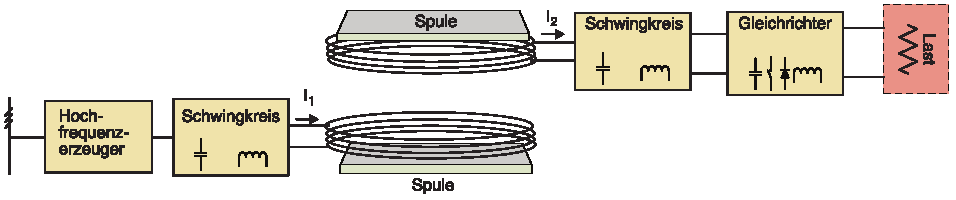
\includegraphics[width=\myFigureStandardWidth]{Resonant-Induktive_Kopplung}
	\caption[Blockdiagramm eines induktiven Ladesystems]{Blockdiagramm eines induktiven Ladesystems. Nach: Chetvorno (Eigenes Werk) CC0, via Wikimedia Commons}
	\label{abb_ResIndKopplung}
\end{figure}

\subsubsection{Statisch}
Bei statischen Ladesystemen lädt der Bus im Stand an Haltestellen oder speziellen Ladestationen. Der Bus wird vom Fahrer anhand von Markierungen auf dem Boden ausgerichtet, teilweise wird die Sekundärspule näher an die Straße abgesenkt. Dadurch kann effizient geladen werden. Es gibt mehrere statische induktive Ladesysteme für Busse, die bereits seit Jahren im Einsatz sind, so zum Beispiel das System \emph{IPT} con \textsc{Conductix-Wampfler} in Turin und das System \emph{primove} von \textsc{Bombardier} in Braunschweig~\cite{WeIPT}. In dieser Arbeit wird das System \textsc{primove} mit 200 kW Ladeleistung betrachtet.

\subsubsection{Dynamisch}
Induktiv-dynamische Ladesysteme können die Batterie während der Fahrt aufladen. Wenn die ganze Strecke ausgerüstet ist kann die Batterie sogar entfallen. Während der Fahrt kommt es durch Lenkfehler zu einer lateralen Abweichung von der Ladestrecke. Die Bewegungen der Federung führen zu einem unterschiedlichen Vertikalen Abstand zwischen den Spulen. Um ein Aufsetzen auf der Straße zu vermeiden muss das System recht hoch im Bus angebracht werden. Dies führt zu einer niedrigen Effizienz~\cite{5618092}. Es werden nur die jeweils direkt unter dem Bus befindlichen Segmente der Primärspule eingeschaltet, was eine Aufteilung der Spule und Schalttechnologie unter der Straße erfordert.

Induktiv-dynamische Systeme könnten zukünftig eine wichtige Rolle in der Elektromobilität spielen, sind jedoch aktuell noch nicht ausgereift genug um einen Stadtbus im Fahrplanverkehr zu versorgen. Von daher werden sie hier nicht weiter betrachtet. 

\subsection{Batteriewechselsysteme}
Im Gegensatz zu den anderen Systemen wird bei Batteriewechselsystemen keine elektrische Energie in das Fahrzeug übertragen sondern die komplette Batterie ausgewechselt. Statt Energietransport findet hier also Stofftransport zwischen Ladestation und Bus statt. 

In aktuellen Systemen werden die Batterien in speziellen Gebäuden durch Roboter ausgetauscht. Innerhalb von kurzer Zeit können so auch sehr große Batterien ausgewechselt werden. Die "`Ladeleistung"' ist sehr groß. Die Batterien können außerhalb des Busses mit optimaler Ladeleistung und bei optimaler Temperatur aufgeladen werden. Es muss jedoch mehr als eine Batterie pro Bus vorgehalten werden, was dieses System sehr teuer macht.\marginpar{Beleg!, Wo wird das eingesetzt}

In dieser Arbeit wird ein in Shanghai eingesetztes Batteriewechselsystem betrachtet\marginpar{stimmts?}. Dieses System kann die Batterie in sieben Minuten austauschen.


\section{Parameter zum Vergleich der Ladesysteme}
\label{parameter}

\subsection{Mechanische Kriterien}
\begin{description}
	\item [Ladestrategie] Ladestrategie, für die dieses System geeignet ist.
	\item [Abmaße, feste Position] \emph{fahrzeug- und stationsseitig}\\
	Die Abmaße jener Komponenten des Ladesystems, deren Postion relativ zu ihrem Gegenüber fest ist.\\
	Beispiel: Pantograph und Stromschiene
	\item [Abmaße, freie Position] \emph{fahrzeug- und stationsseitig}\\
	Die Abmaße jener Komponenten des Ladesystems, deren Postion frei gewählt werden kann.\\
	Beispiel: Elektrische Wandler
	\item [Masse] \emph{fahrzeugseitig}\\
	Gesamtmasse der fahrzeugseitigen Komponenten
	\item [Freiheitsgrade] \emph{fahrzeug- und stationsseitig}\\
	Anzahl der Freiheitsgrade, die eine bewegliche Komponente relativ zum Fahrzeug oder zur Station hat. 0, wenn es keine beweglichen Teile gibt.
	\item [Positionierungsgenauigkeit des Busses] \emph{fahrzeugseitig} \\
	Erforderliche Genauigkeit der Positionierung des Busses relativ zur Ladestation, so dass die volle Ladeleistung verfügbar ist. Besteht aus zwei translatorischen und einer rotatorischen Komponente (X, Y, Richtung des Busses)
	\item [Totzeit]
	Summe aus Zeit zwischen Halt des Busses und Ladebeginn sowie Zeit zwischen Ladeschluss und Abfahrt. Ist die Zeit von der Position abhängig, so wird jeweils eine Abweichung um die Hälfte des maximalen Wertes angenommen.
	\item [Anzahl der Wandler] \emph{fahrzeug- und stationsseitig}\\
	Anzahl der Komponenten, die den Spannungsverlauf verändern (Gleichrichter, Transformatoren etc.)
\end{description}

\subsection{Elektrische Kriterien}
\begin{description}
	\item [Leistung]
	Aus dem öffentlichen Stromnetz erforderliche Leistung. Die im Bus angekommene Leistung ergibt sich durch die Effizienz. Es wird angenommen, das die Leistung aus dem ortsüblichen Niederspannungsnetz kommt. (400V Drehstrom in Europa)\marginpar{Amerika}
	\item [Effizienz]
	Prozentualer Anteil der Leistung, die im Fahrzeug am Laderegler des Energiespeichers ankommt.		
\end{description}

\subsection{Sicherheit}
\begin{description}
	\item [Exponierte Leiter]
	Sind die spannungsführenden Leiter nur durch die umgebende Luft isoliert? Mögliche Antworten: nie, nur beim Ladevorgang, immer
	\item [Zugänglichkeit der Schnittstelle]
	Wo am Fahrzeug ist die Ladeschnittstelle? Wie ist sie geschützt?
	\item [Position der Ladestation]
	Ladesäule oder Unterflur? Im Depot oder an öffentlich zugänglicher Station?	
\end{description}


\section{Wertetabellen}
\label{sec_tabellen_ladesysteme}
\marginpar{Methodik!}
\FloatBarrier
\subsection{Mechanische Kriterien}
%%%% MECHANISCHE TABELLEN %%%%
\begin{table}[h!]\centering
	\begin{tabularx}{\textwidth}{lXlr}
		\toprule
		System                         & Kurzname & Ladestrategie        & Totzeit \\
		                               &          &                      & $s$     \\ \midrule
		1x \textsc{IEC 62196-2}        & 40kW     & Nacht  & \emph{60} \\
		\textsc{primove}               & 200kW    & Gelegenheitsladen    & 4 \\
		\textsc{Schunk Smart Charging} & 375kW    & Gelegenheitsladen    & 8 \\
		Batteriewechsel                & Swap     & Nacht \& Gelegenheit & 420 \\ \bottomrule
	\end{tabularx}
	\caption[Allgemeine mechanische Kriterien Ladesysteme]{Allgemeine mechanische Kriterien Ladesysteme. \emph{Kursive} Werte sind geschätzt}
	\label{tab_mech_Ladesys_allg}
\end{table}

\begin{table}[h!]\centering
	\begin{tabularx}{\linewidth}{Xlllll}
		\toprule
		System & Maße fest & Maße frei  & Masse     & Freiheitsgrade & Genauigkeit            \\
		       & $l$       & $l$        & $kg$      & $1$            & $m^2,^{\circ}$         \\ \midrule
		40kW   & 0         & \emph{50}  & \emph{50} & 0              & 47$m^2$, 360$^{\circ}$ \\
		200kW  & 198       & \emph{100} & 450       & 1              & ???                    \\
		375kW  & 1000      & \emph{100} & 185       & 3              & 1,75$m^2$, 2$^{\circ}$ \\
		Swap   & 0         & 0          & 0         & 0              & unbekannt             \\ \bottomrule
	\end{tabularx}
	\caption[Mechanische Kriterien der Ladesysteme – fahrzeugseitig]{Mechanische Kriterien der Ladesysteme – fahrzeugseitig. \emph{Kursive} Werte sind geschätzt}
	\label{tab_mech_Ladesys_fzg}
\end{table}

\begin{table}[h!]\centering
	\begin{tabularx}{\linewidth}{Xrrrr}
		\toprule
		System & Maße fest &   Maße frei & Freiheitsgrade & Wandler \\
		       &       $l$ &         $l$ &            $1$ &     $1$ \\ \midrule
		40kW   &         0 &          88 &              0 &      ?? \\
		200kW  &      1800 & \emph{2000} &              0 &      ?? \\
		375kW  &       325 & \emph{2000} &              0 &      ?? \\
		Swap   &         0 & $\gg10.000$ &           $>2$ &      ?? \\ \bottomrule
	\end{tabularx}
	\caption{Mechanische Kriterien der Ladesysteme – stationsseitig}
	\label{tab_mech_Ladesys_stat}
\end{table}
\FloatBarrier

\subsection{Elektrische Kriterien}
%%%% ELEKTRISCHE TABELLE %%%%
\begin{table}[h!]\centering
	\begin{tabularx}{\linewidth}{XXX}
		\toprule
		System & Leistung & Effizienz \\
		       & $kW$     & $\%$      \\ \midrule
		40kW   & 40       & \emph{99} \\
		200kW  & 200      & 95 \\
		375kW  & 375      & \emph{99} \\
		Swap   & $\infty$ & \emph{99} \\ \bottomrule
	\end{tabularx}
	\caption{Elektrische Kriterien der Ladesysteme}
	\label{tab_el_Ladesys}
\end{table}
\FloatBarrier

\subsection{Zuverlässigkeit}

%%%% SICHERHEIT %%%%
\begin{table}[h!]\centering
	\begin{tabularx}{\linewidth}{XXXX}
		\toprule
		System         & Exponierte Leiter & \multicolumn{2}{c}{Zugänglichkeit Schnittstelle} \\
		\cmidrule{3-4} &                   & Ladestation  & Fahrzeug                          \\ \midrule
		40kW           & nie               & Bodenhöhe    & Bodenhöhe                         \\
		200kW          & nie               & Unterflur    & Unterseite                        \\
		375kW          & nur beim Laden    & Eröht        & Dach                              \\
		Swap           & nie               & Unzugänglich & Bodenhöhe                         \\ \bottomrule
	\end{tabularx}
	\caption{Sicherheitskriterien der Ladesysteme}
	\label{tab_sich_Ladesys}
\end{table}
\FloatBarrier



